\documentclass[10pt,oneside,a4paper]{article}
\usepackage[margin=0.5in]{geometry} 
% \usepackage[a4paper,landscape, margin=0.5in]{geometry} % Add landscape option
\usepackage{enumitem}
\usepackage{xcolor}
\usepackage{todonotes}
\usepackage{amsmath}
\usepackage{caption}
\usepackage{hyperref}
\usepackage{graphicx}
\usepackage{listings}
\usepackage{amssymb}
\usepackage{bbm}
\usepackage{float}
\usepackage{algorithm}
\usepackage{algorithmic}
% \usepackage{multicol}

\begin{document}
% \begin{multicols}{2}

\paragraph{Association rule mining}
Rule strength measure
\[
    \text{support}(X \rightarrow Y) = \frac{\text{count}(X \cup Y)}{n}
\]
\[
    \text{confidence}(X \rightarrow Y) = \frac{\text{count}(X \cup Y)}{\text{count}(X)}
\]

\section{Apriori frequent itemset algorithm}
init-pass obtains the items in lexicographic order.
\begin{figure}[H]
    \centering
    \begin{minipage}[t]{0.5\textwidth}
        \centering
        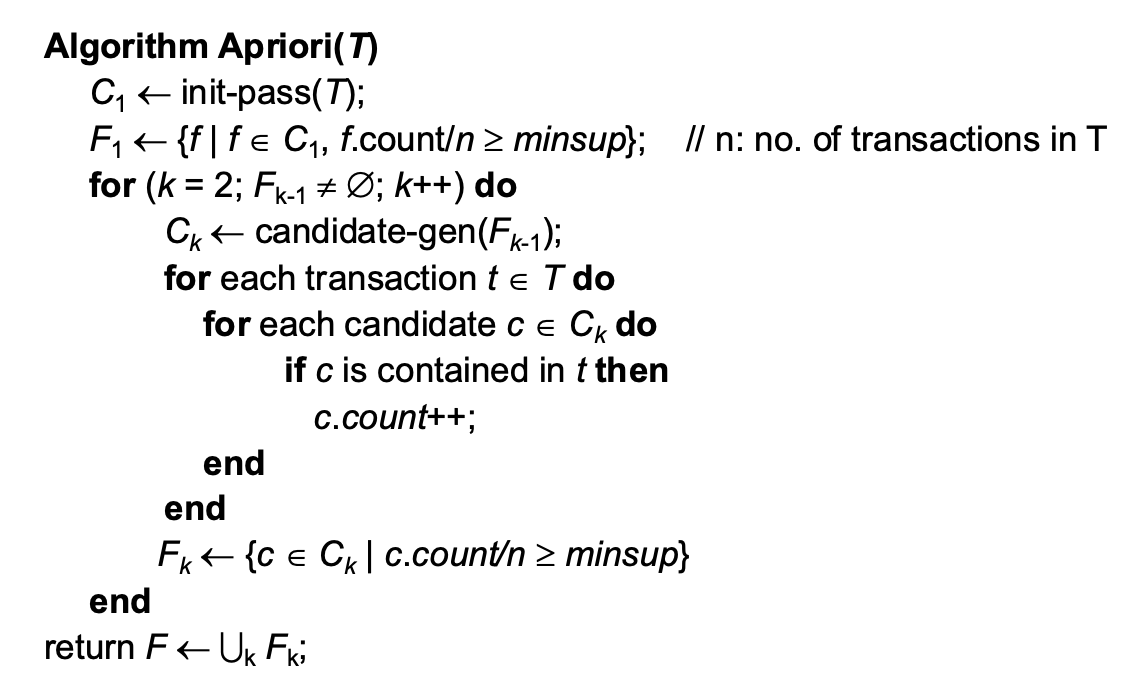
\includegraphics[width=0.8\textwidth]{Images/Apriori.png}
    \end{minipage}%
    \hfill
    \begin{minipage}[t]{0.5\textwidth}
        \centering
        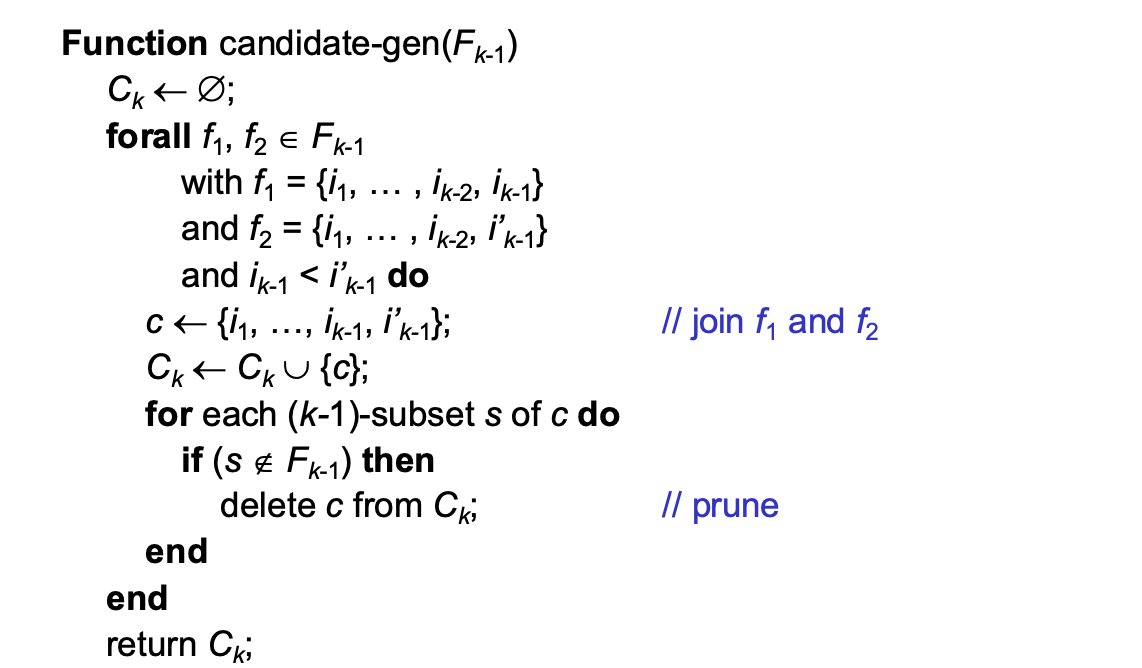
\includegraphics[width=0.8\textwidth]{Images/Candidate_gen_apriori.png}
    \end{minipage}%
\end{figure}

\section{MS Apriori}
sort in ascending
\begin{figure}[H]
    \centering
    \begin{minipage}[t]{0.32\textwidth}
        \centering
        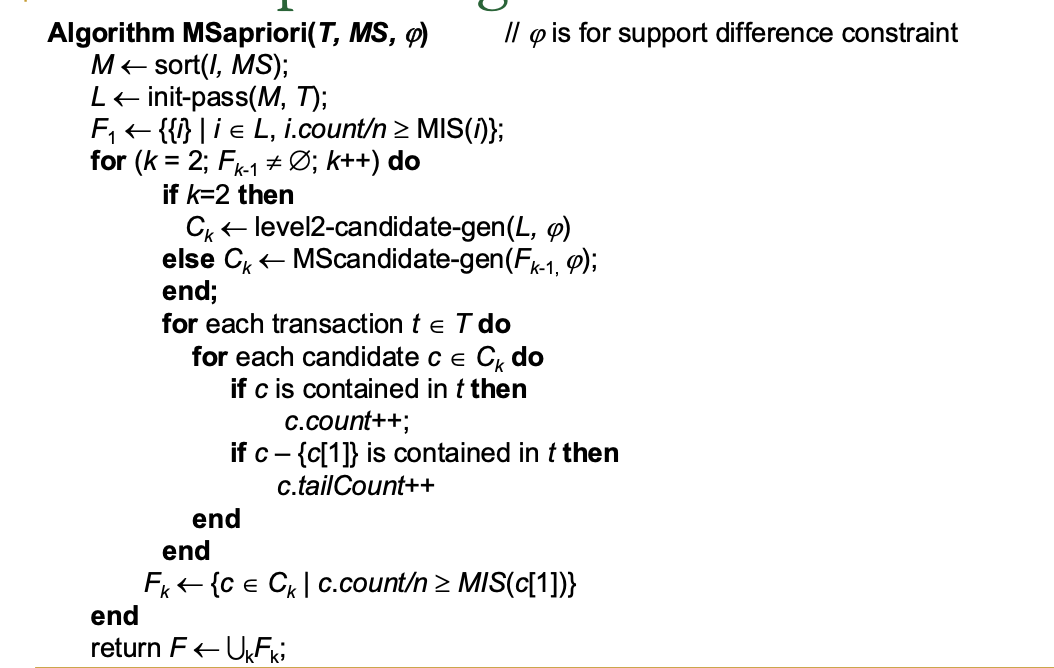
\includegraphics[width=\textwidth]{Images/MsApriori.png}
        \caption{MsApriori}
    \end{minipage}%
    \hfill
    \begin{minipage}[t]{0.32\textwidth}
        \centering
        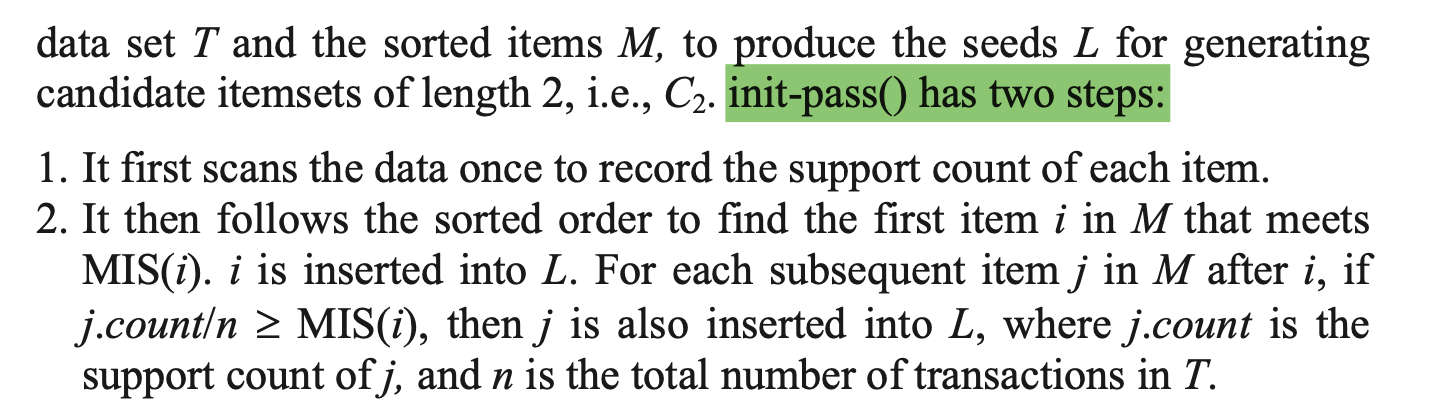
\includegraphics[width=\textwidth]{Images/init_pass.png}
        \caption{Init Pass}
    \end{minipage}%
    \hfill
    \begin{minipage}[t]{0.32\textwidth}
        \centering
        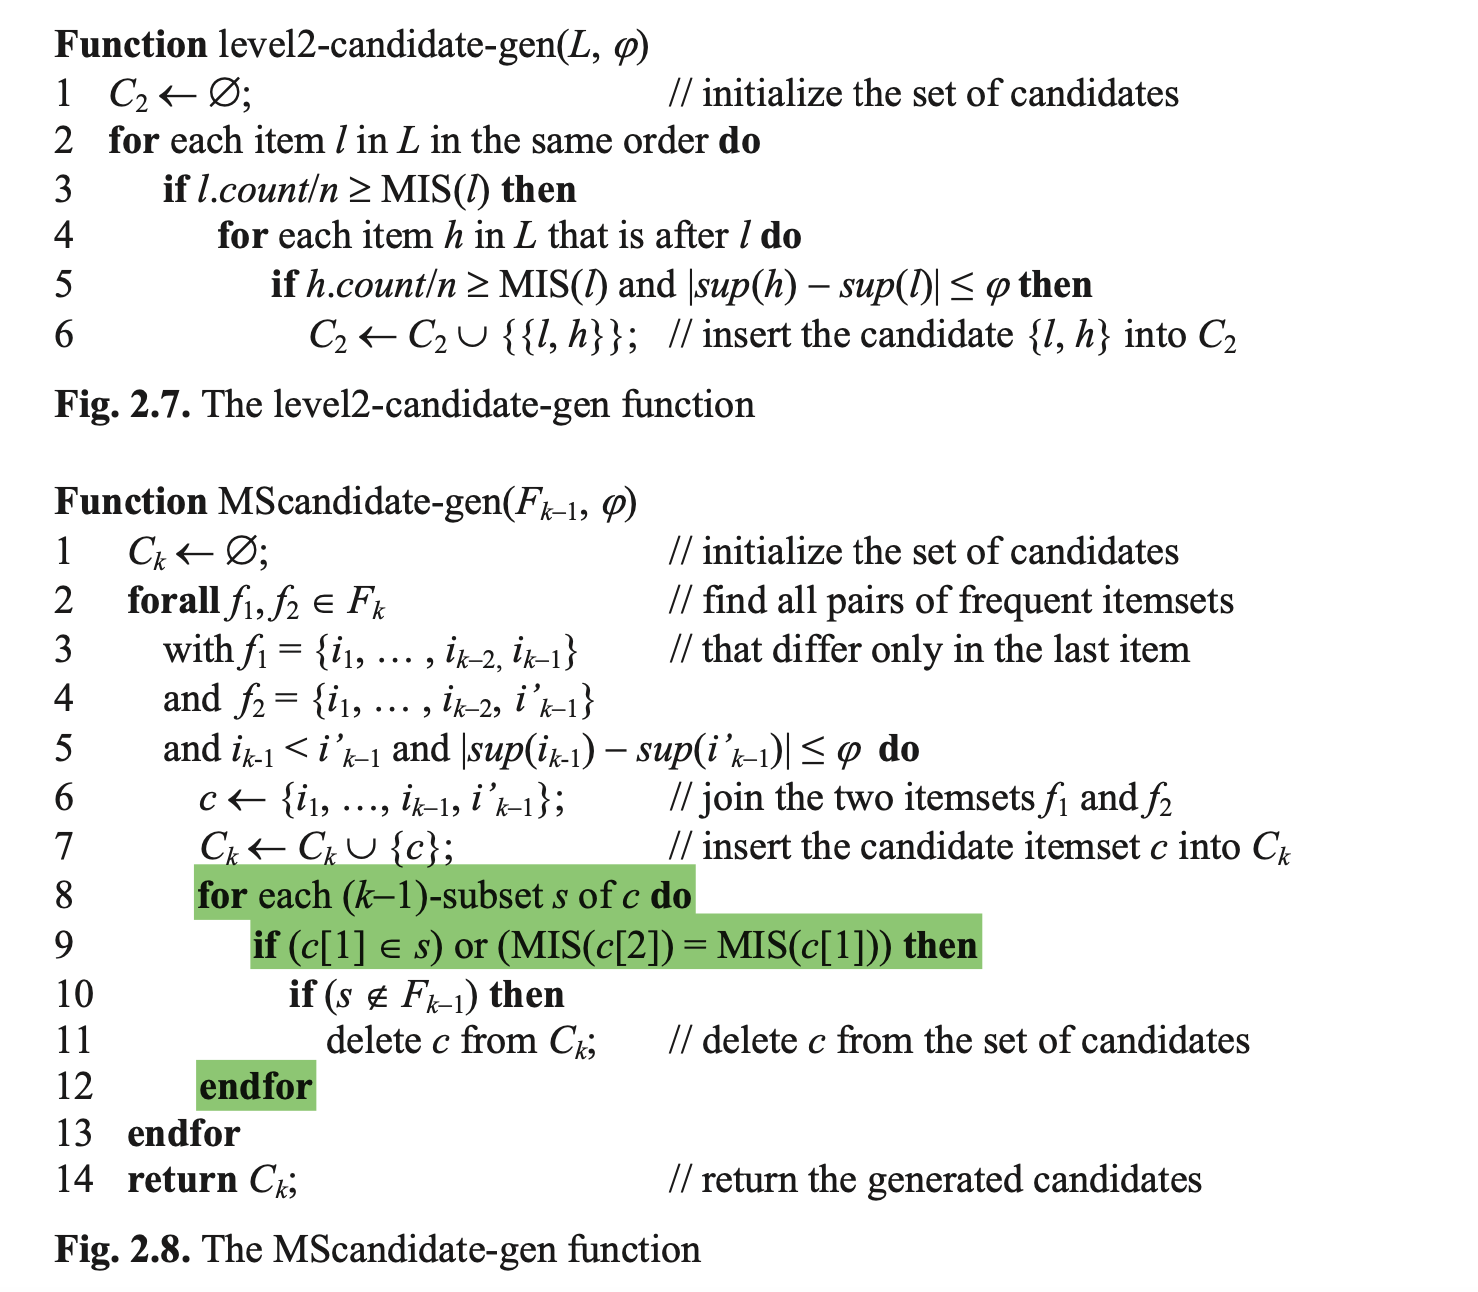
\includegraphics[width=\textwidth]{Images/Candidate_gen_MS.png}
        \caption{Candidate Gen MS}
    \end{minipage}
\end{figure}


\section{GSP (sequential pattern mining)}
\begin{figure}[H]
    \centering
    \begin{minipage}[t]{0.5\textwidth}
        \centering
        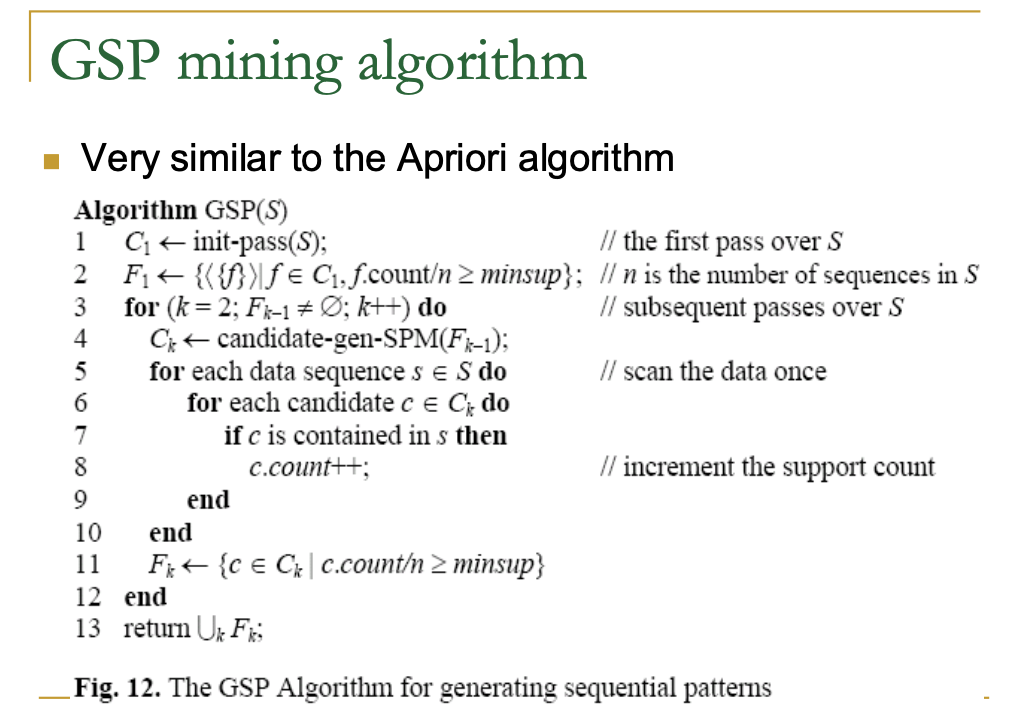
\includegraphics[width=0.8\textwidth]{Images/GSP1.png}
    \end{minipage}%
    \hfill
    \begin{minipage}[t]{0.5\textwidth}
        \centering
        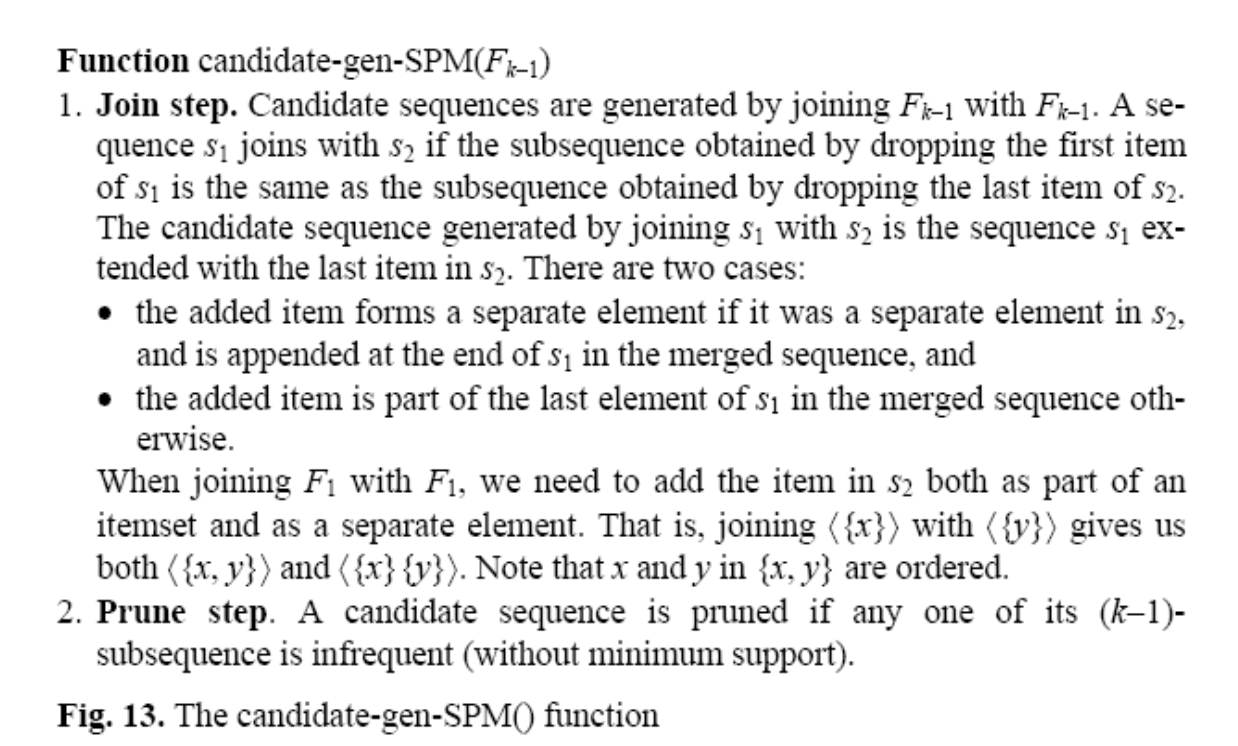
\includegraphics[width=0.8\textwidth]{Images/GSP.png}
    \end{minipage}%
\end{figure}
When he says is the same as the subsequence... Means that you have to remove the parenthesis and see if the elements are in the same order.

\section{Index for Classifiers}

\begin{table}[H]
    \centering
    \begin{tabular}{|l|l|}
        \hline
        \textbf{Metric}           & \textbf{Description / Formula}                                       \\ \hline
        Accuracy                  & $\frac{\text{Correctly Classified Examples}}{\text{Total Examples}}$ \\ \hline
        Precision                 & $\frac{TP}{TP + FP}$: Of predicted positives, how many are correct.  \\ \hline
        Recall/sensitivity (TPR)  & $\frac{TP}{TP + FN}$: Of actual positives, how many are identified.  \\ \hline
        $F_1$ Score               & $2 \times \frac{p \cdot r}{p + r}$: Combines precision and recall.   \\ \hline
        Specificity (TNR)         & $\frac{TN}{TN + FP}$: True negative rate.                            \\ \hline
        False Positive Rate (FPR) & $1 - \text{TNR}$                                                     \\ \hline
        ROC Curve                 & Plot: FPR (x-axis) vs. TPR (y-axis).                                 \\ \hline
    \end{tabular}
    \caption{Summary of Classification Metrics}
\end{table}


\section{Decision trees}
\begin{figure}[h!]
    \centering
    \begin{minipage}{0.5\textwidth}
        \centering
        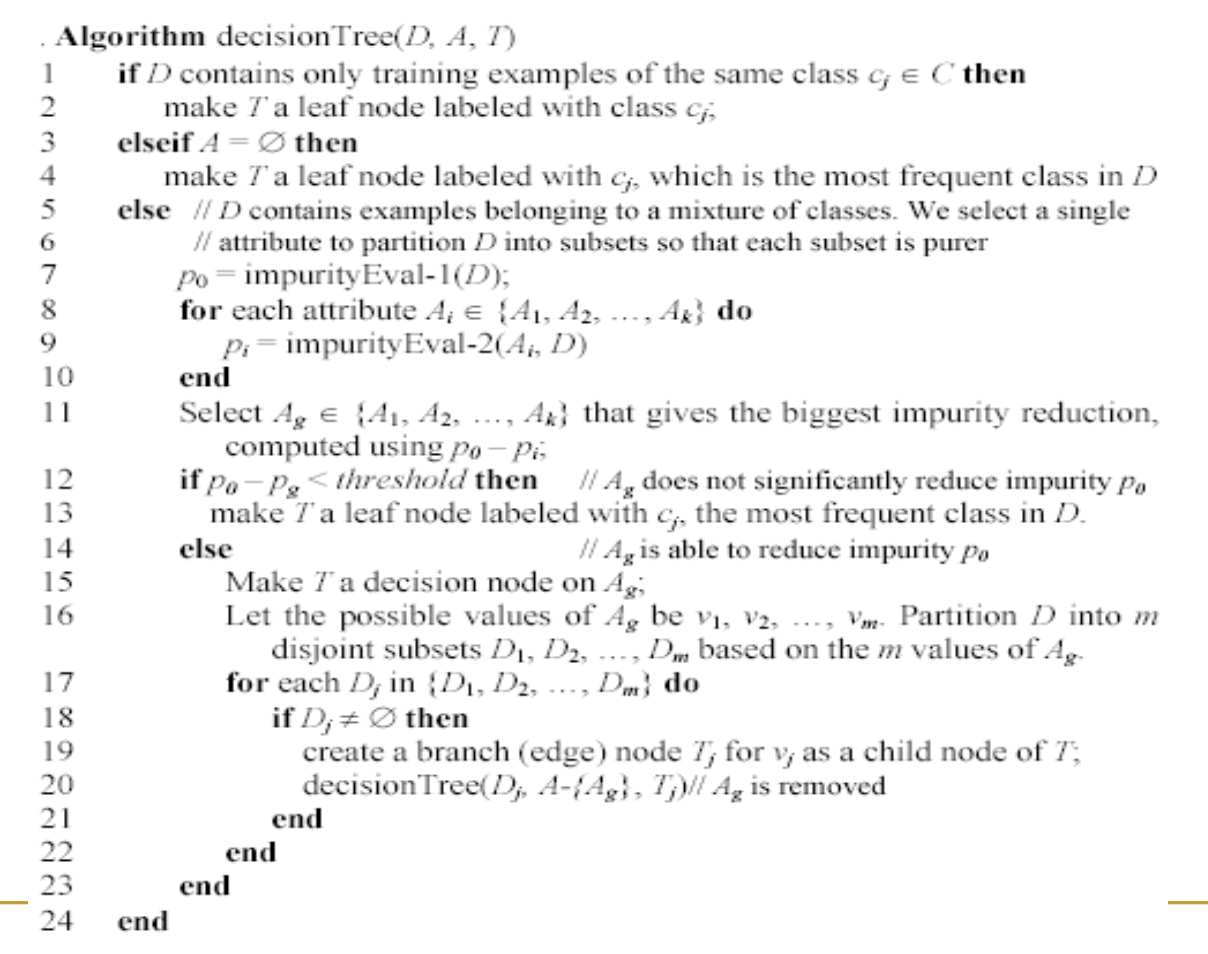
\includegraphics[width=0.8\textwidth]{Images/DecisionTree.png}
    \end{minipage}%
    \hfill % Optional space between the image and text
    \begin{minipage}{0.5\textwidth}
        \paragraph{Entropy}
        D is the dataset. C are the different classes in the dataset.

        \[
            \text{entropy}(D) = - \sum_{j=1}^{|C|} \text{Pr}(C_j) \log_2 \text{Pr}(C_j)
        \]

        Is a positive value.
        The sum of the probabilities of the classes is 1.
        The more the data is purer, the more the entropy value is close to zero.
        Worst entropy is 1 (all the classes are equally distributed).

        \[
            \text{entropy}_{A_i}(D) = \sum_{j=1}^{v} \frac{|D_j|}{|D|} \times \text{entropy}(D_j)
        \]

        This value is the entropy if we choose to partition the data over attribute A. There are v possible values for the attribute A.
        Entropy$(D_j)$ is the entropy in the subset of data that has the value $v_j$ for the attribute A.

        \[
            \text{gain}(D, A_i) = \text{entropy}(D) - \text{entropy}_{A_i}(D)
        \]
        The higher the gain the better

    \end{minipage}
\end{figure}


\section{Naive based classification}
\begin{figure}[H]
    \centering
    \begin{minipage}{0.5\textwidth}
        \centering
        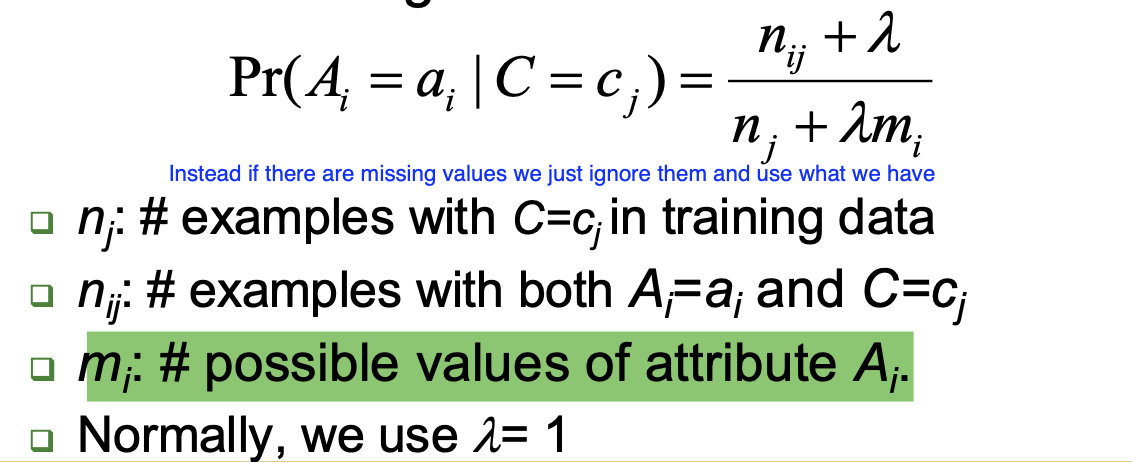
\includegraphics[width=0.8\textwidth]{Images/Zerocounts.png}
    \end{minipage}%
    \hfill % Optional space between the image and text
    \begin{minipage}{0.5\textwidth}
        Product rule
        \[
            \text{Pr}(a1, a2) = \text{Pr}(a1) \text{Pr}(a2 | a1)
        \]
        Product rule for conditional probability
        \[
            \text{Pr}(a1, a2|c) = \text{Pr}(a2|c) \text{Pr}(a2 | a1, c)
        \]
        General case
        \[
            \text{Pr}(a_1 \cdots a_n \mid c) = \text{Pr}(a_1 \mid c) \text{Pr}(a_2 \mid c, a_1) \cdots \text{Pr}(a_n \mid c, a_1 \cdots a_{n-1})
        \]
        Conditional independence assumption
        \[
            \text{Pr}(a_i \mid c, a_1 \cdots a_{i-1}) = \text{Pr}(a_i \mid c)
        \]
        Goal:
        \[
            \text{Pr}(c \mid (a_1 \cdots a_n)) = \frac{\text{Pr}(c)  \text{Pr}((a_1 \cdots a_n) \mid c)}{\text{Pr}(a_1 \cdots a_n)}
        \]
        Using the law of total probability
        \[
            \text{Pr}(a_1 \cdots a_n) = \sum_{r=1}^{|C|} \text{Pr}(c) \text{Pr}((a_1  \cdots a_n) \mid c)
        \]
        Using the product rule and the conditional independence assumption
        \[
            \text{Pr}(c \mid (a_1 \cdots a_n)) = \frac{\text{Pr}(c) \prod_{i=1}^{n} \text{Pr}(a_i \mid c)}{\sum_{r=1}^{|C|} \text{Pr}(c) \prod_{i=1}^{n} \text{Pr}(a_i \mid c)}
        \]

        Adjusting the probability to account for attribute values that don't occur with that class.

    \end{minipage}
\end{figure}

\begin{figure}[H]
    \centering
    \begin{minipage}{0.5\textwidth}
        \section{Naive based text classification}

        \[
            \text{Pr}(c | d) = \frac{\text{Pr}(c) \text{Pr}(d|c)}{\text{Pr}(d)}
        \]
        \[
            = \frac{\text{Pr}(c) \prod_{k=1}^{\text{all word in d}} \text{Pr}(w_k|c)}{\sum_{r=1}^{|C|} \text{Pr}(c_r) \prod_{k=1}^{\text{all word in d}} \text{Pr}(w_k|c)}
        \]
        \[
            \text{Pr}(c) = \frac{\sum_{i=1}^{|D|} \text{Pr}(c|d_i)}{|D|}
        \]
        \[
            \text{Pr}(w_k|c) = \frac{\sum_{i=1}^{|D|} N_{ik} \text{Pr}(c|d_i)}{\sum_{s=1}^{|V|} \sum_{i=1}^{|D|} N_{si} \text{Pr}(c|d_i)}
        \]
        $N_{ij}$ is the number of times that the word j appears in a document i.
    \end{minipage}%
    \hfill % Optional space between the image and text
    \begin{minipage}{0.5\textwidth}
        \section{K-means}
        \centering
        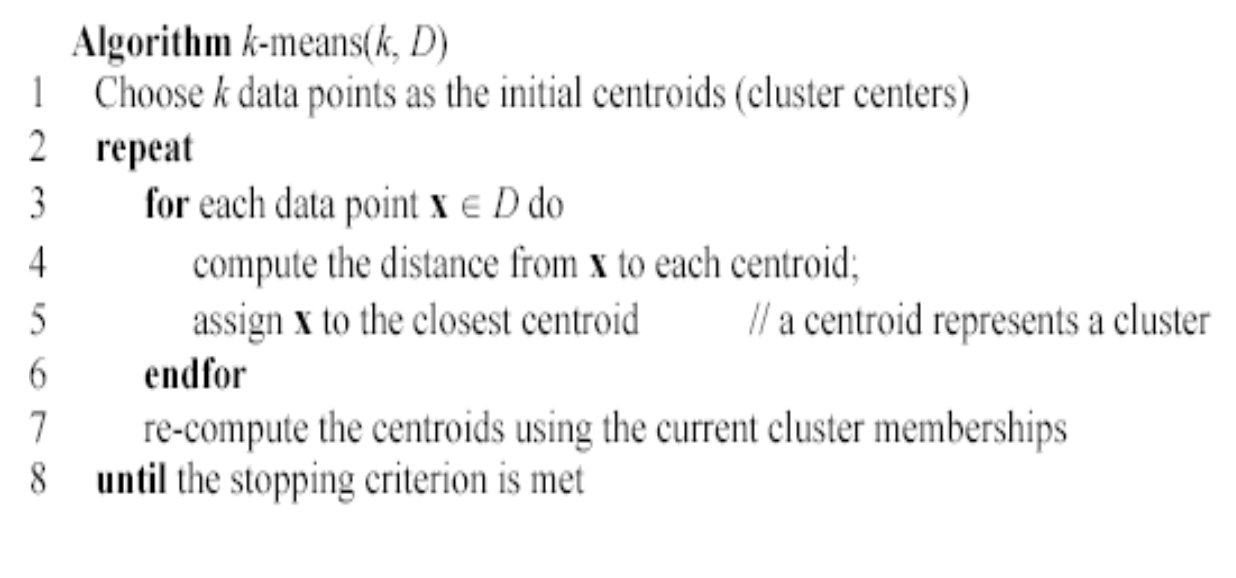
\includegraphics[width=0.5\textwidth]{Images/kmeans.png}

    \end{minipage}
\end{figure}

\begin{figure}[H]
    \centering
    \begin{minipage}{0.5\textwidth}
        \section{Agglomerative clustering}

        \centering
        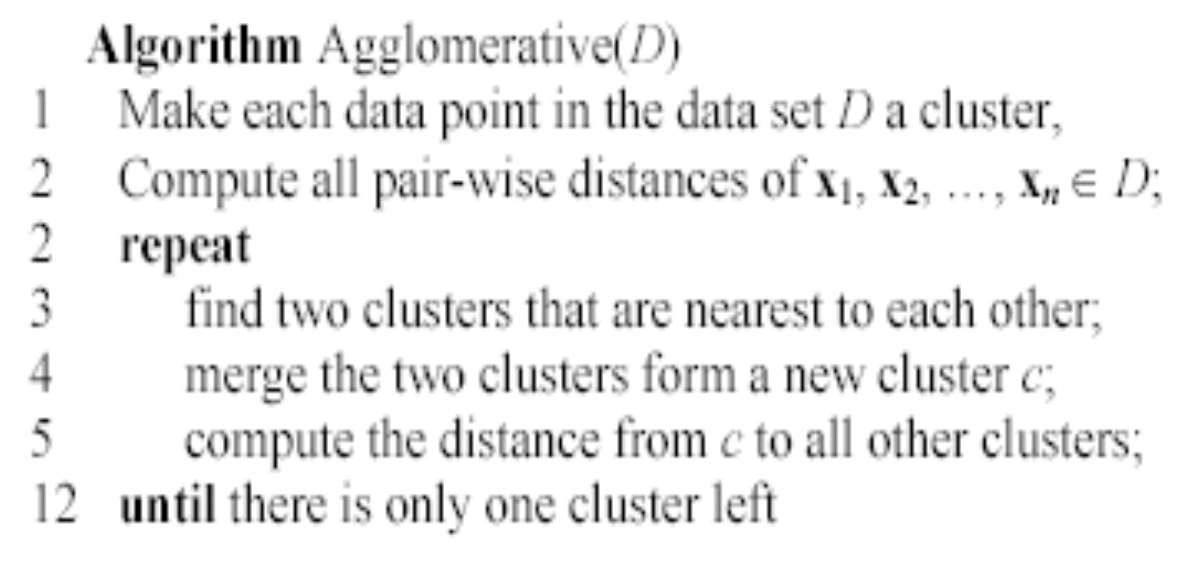
\includegraphics[width=0.5\textwidth]{Images/Agglomerative_clustering.png}
    \end{minipage}%
    \hfill % Optional space between the image and text
    \begin{minipage}{0.5\textwidth}
        Distance metrics:
        \begin{itemize}
            \item Single link: distance between two clusters is the distance between two closest data points in the two clusters.
            \item Complete link: distance between two clusters is the distance of two furthest data points in the two clusters.
            \item Average link: average distance between all points in the two clusters. (most precise metrics but also most computationally expensive)
            \item Centroid link: distance between the centroids of the two clusters. (doesn't consider the shape of the cluster)
        \end{itemize}

    \end{minipage}
\end{figure}
\begin{figure}[H]

\end{figure}




\section{LU learning}



\section{Search Engines}

\subsection{Transition Probability Matrix}
Transition probability matrix:
\[
    A_{i,j} =
    \begin{cases}
        \frac{1}{\text{outdegree}(i)} & \text{if there is a link from } i \text{ to } j, \\
        0                             & \text{otherwise.}
    \end{cases}
\]
stochastic matrix: the sum of the elements in each row is 1.

we make stochastic by assigning an equal probability to each link for rows that are all zeros. or by removing the node without outgoing edges.

\paragraph{Irreducible}
An adjacency matrix is irreducible if the graph it represents is \emph{strongly connected}, meaning there is a path between every pair of nodes in the graph.

\paragraph{Aperiodic}
A state \( i \) in a Markov chain is periodic with period \( k > 1 \) if \( k \) is the smallest number such that all paths leading from state \( i \) back to state \( i \) have a length that is a multiple of \( k \).

A graph is \emph{aperiodic} if there are no cycles that you cannot escape from.

\paragraph{Making the Matrix Aperiodic and Irreducible}
To ensure the matrix is both aperiodic and irreducible We assign a small probability that the user will jump to a random page. (we add a damping factor)

\paragraph{Final formula for page rank}
\[
    P = (1 - d)e + dA^T P
\]

\section{Finding holes}
Use tree. Add uniformly sampled points with class Hole. Perform the regular decision tree.
We add a different number of \( N \) points at each node.

\begin{itemize}
    \item The number of \( N \) points for the current node \( E \) is determined by the following rule (note that at the root node, the number of inherited \( N \) points is \( 0 \)):
\end{itemize}

\begin{enumerate}
    \item If the number of \( N \) points inherited from the parent node of \( E \) is less than the number of \( Y \) points in \( E \), then:
          \begin{itemize}
              \item The number of \( N \) points for \( E \) is increased to the number of \( Y \) points in \( E \).
          \end{itemize}
    \item Else:
          \begin{itemize}
              \item The number of inherited \( N \) points is used for \( E \).
          \end{itemize}
\end{enumerate}

\section{EM (expectation maximization)}
Train a classifier with only the labeled
documents. Use it to probabilistically classify the
unlabeled documents. Use ALL the documents to train a new
classifier. Iterate steps 2 and 3 to convergence.


\section{Recommender systems}
Matrix factorization
Users and movies are categorized in a latent space that is composed by a fixed number of features (could be the genre, star actor). We obtain two matrixes, one for users and one for movies. The probability that an user likes the movie is the sum of product of the user and movie features.

\[
    P_{i,j} = U_i^T \cdot M_y
\]

Where U and I are column vectors.

The learning rule is
\[
    u_{ki}^{t+1} = u_{ki}^t + 2\gamma (r_{ij} - p_{ij})m_{kj}^t
\]

\[
    m_{kj}^{t+1} = m_{kj}^t + 2\gamma (r_{ij} - p_{ij})u_{ki}^t
\]

\section{Sentiment quintuple}
Holder, time, entity, aspect, sentiment.


\section{General definitions}
\textbf{Continual learning}: Continual learning is the ability of a model to learn new tasks incrementally without forgetting previously
learned tasks.
\textbf{Class-incremental learning}: Class-incremental learning involves learning new classes incrementally while retaining the ability to
classify previously learned classes.
\textbf{Task-incremental learning}: Task-incremental learning involves learning new tasks sequentially, where task identity is provided
during inference.
\textbf{Inter-task class separation}: Inter-task class separation refers to maintaining distinct boundaries between classes from different
tasks to prevent interference.
\textbf{Objectives of continual learning}: The two main objectives are avoiding catastrophic forgetting and promoting knowledge
transfer between tasks.
\textbf{Closed world learning}: Closed world learning assumes the model only encounters data belonging to predefined classes.
\textbf{Open-world learning, on-the-job learning, and continual learning after deployment}: These involve learning from data
incrementally after deployment, adapting to new classes, and handling open-set scenarios.
\textbf{Out-of-distribution detection}: Out-of-distribution detection identifies inputs that differ significantly from the training data's
distribution.
\textbf{CML (Continual Meta-Learning)}: CML enables a model to quickly adapt to new tasks using prior knowledge while mitigating
forgetting.
\textbf{Self-initiated open-world continual learning and adaptation}: This framework involves a model autonomously identifying and
learning from novel classes in an open-world scenario
\end{document}